
{\color{red} \bf Warning:}
The findings and conclusions in this article have not been
formally disseminated
and should not be construed to represent any determination or
policy of University, Agency, and National Laboratory.

This document is written to explain the main
functions of \pkg{cubfits}~\citep{Chen2014cubfitspackage}, version 0.1-2.
Every effort will be made to ensure future versions are consistent with
these instructions, but features in later versions may not be explained
in this document.




\section[Introduction]{Introduction}
\label{sec:introduction}
\addcontentsline{toc}{section}{\thesection. Introduction}

Coding sequences or open reading frames (ORFs) are regions of genome encoding
proteins required to properly function any living biological organism.
In order to adopt to environment, growth in limited resource, or
maintain population size, the protein production needs to be reflect quickly
under those condition. The efficiency of protein translation is essentially
critical for some tiny organism, such as yeast.
For example, we may model the translation rates,
from a codon sequence to a protein,
with several factors and in several ways.
Once the codon information
encoded behind a genome is estimated/approximated appropriately, then
the model can be used to predict gene expression levels or protein production
rates. Therefore, it is interesting
to know what factors may affect production rates, how strong they are, or
whether genomes evolve accordingly.

In a simplified example, Cysteine (Cys/C) is one of 20 amino acids and
can be encoded by two synonymous codons, TGT and TGC. Suppose Cysteine are
observed in two coding sequences and used to encode two proteins.
Suppose further one has lower expression level, but the other one has higher
expression level. Assume TGT and TGC both have no effect to expression level,
then the chance of observing TGT and TGC is roughly 50\% and 50\% among
both coding sequences. Suppose the chance of observing TGC is much higher
than observing TGT in the protein has higher expression level, then we
may guess that TGT is more efficient than TGC for that protein translation.

\pkg{cubfits}~\citep{Chen2014cubfitspackage} models the biased patterns of codon usage among other
information and fits model parameters. The implemented models are introduced
in \citep{Gilchrist2007,Shah2011,Wallace2013}
that combines several
modeling techniques of Population Genetics and Statistics to
predict protein production rates.

Package requirements and installation of \pkg{cubfits} are described
next. Section~\ref{sec:main_functions} gives short examples for
main functions.
Section~\ref{sec:speedup} provides parallel implementations that simply
speedup computations, and discusses technical issues.
In Section~\ref{sec:work_flows}, useful work flows
built in \pkg{cubfits} are introduced.
Section~\ref{sec:utilities} introduces implemented methods of data
input/output and conversion between different data structures with examples.
Finally, Section~\ref{sec:misc} introduces some useful functions.


\subsection[Requirements]{Requirements}
\addcontentsline{toc}{subsection}{\thesubsection. Requirements}

\pkg{cubfits} is a package of \proglang{R}~\citep{Rcore} built and test on
\proglang{R} 3.0.0, but may be compatible back to 2.15.0 or early.
It requires \pkg{methods} package which is default in \proglang{R}, and
suggests \pkg{seqinr}~\citep{seqinr} and \pkg{VGAM}~\citep{VGAM}
packages that both are available and
can be installed from CRAN or it's mirror sites.
The \pkg{seqinr} takes care input and output of DNA sequence data
in FASTA format, and the \pkg{VGAM} takes care several core functions of
model fitting used by \pkg{cubfits}.
The \pkg{cubfits} also uses several high performance computing
techniques to speed up computation including
\pkg{parallel}~\citep{parallel} and
\pkg{pbdMPI}~\citep{Chen2012pbdMPIpackage}.
Further, the \pkg{cubfits} provides some diagnoses for multiple chains of
MCMC results and restart MCMC chains utilizing packages such as
\pkg{doSNOW}~\citep{doSNOW} and \pkg{coda}~\citep{coda}, and
their dependent packages.
Other utilities in \pkg{cubfits} also include
\pkg{EMCluster}~\citep{EMCluster} for a mixture distribution in
one dimension.

The \pkg{cubfits} uses a core function \proglang{vglm()} of \pkg{VGAM} for
model fitting, and (optionally) parallelizes
via \proglang{mclapply()} of \pkg{parallel} package and
\proglang{task.pull()} or \proglang{pbdLapply()} of \pkg{pbdMPI} package.
The parallelization is designed across the 20 amino acids.
Note that \proglang{mclapply()} is only supported on Unix-like systems
and on shared memory machines, while \proglang{tak.pull()} and
\proglang{pbdLapply()} are supported on most systems (Linux/Unix/MacOS/Windows)
and on both of shared memory machines and distributed clusters
provided a MPI~\citep{MPI1994} library is installed.
See \citet{Chen2012pbdMPIvignette} for more details of installation of a
MPI library and \pkg{pbdMPI}.


\subsection[Installation and Test]{Installation and Test}
\addcontentsline{toc}{subsection}{\thesubsection. Installation and Test}

The \pkg{cubfits} can be either installed within an \proglang{R} session as
\begin{Code}
> install.packages("seqinr")
> install.packages("VGAM")
> install.packages("doSNOW")
> install.packages("coda")
> install.packages("EMCluster")
> install.packages("cubfits")
\end{Code}
or installed from a command line as
\begin{Command}
$ R CMD INSTALL seqinr_3.7-0.tar.gz
$ R CMD INSTALL VGAM_0.3-9.tar.gz
$ R CMD INSTALL doSNOW_1.0.12.tar.gz
$ R CMD INSTALL coda_0.16-1.tar.gz
$ R CMD INSTALL EMCluster_0.2-4.tar.gz
$ R CMD INSTALL cubfits_0.1-0.tar.gz
\end{Command}
provided other requirements or dependent packages are installed correctly.
Note that \pkg{parallel} and \pkg{pbdMPI} are optional.

A simple test can be used to see if the \pkg{cubfits} installed correctly
as
\begin{Code}
> demo(plotbin, 'cubfits')
\end{Code}
within an \proglang{R} session, and this demo provides a plot as in
Figure~\ref{fig:plotbin}.
\begin{figure}[ht]
\centering
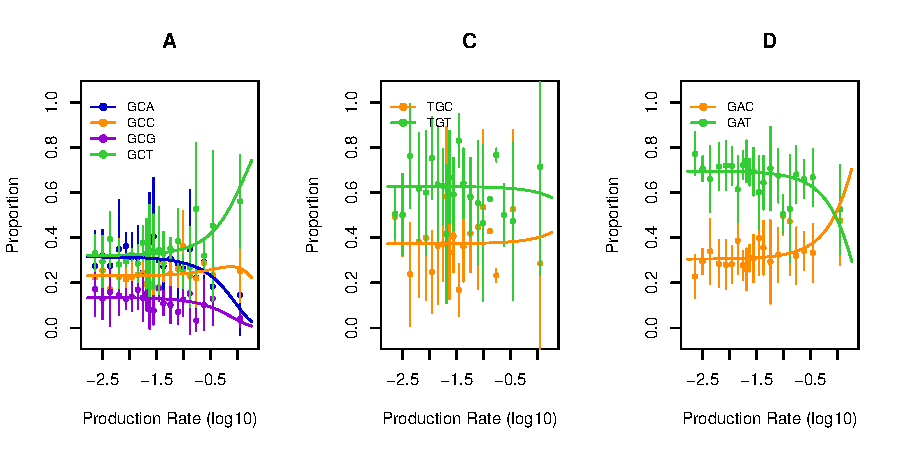
\includegraphics[width=6in]{cubfits-include/figure/plotbin}
\caption{A simple demo plot. Figures show the empirical binning results
by expression levels where dots are mean proportions of synonymous codons
of 100 sequences in every 5\% expression windows, and horizontal lines
are 90\% empirical intervals. The curves are theoretical prediction of
synonymous codon usages~\citep{Shah2011}. See Section~\ref{sec:misc} for
details.
For amino acid A, the selection effect dominates the mutation effect for
some codons at expression level larger than $-1.5$. For C,
it is mainly mutation effect. For D, the selection effect can be
observed at expression level larger than $-0.75$.
}
\label{fig:plotbin}
\end{figure}
